% !TEX root = main.tex
\chapter{System overview}\label{cha:systemOverview}

 First of all, a brief description of the whole collimator will be given is this chapter. This will be followed by a more detailed description of the rotational stage.

\section{Crystal collimators}
A collimator is a specially designed device, built to interfere with the beam and clean it from surrounding halo particles. To be able to meet the future demand of higher energy levels, a more efficient collmator is being devloped at CERN. This new collimator will utilze a crystaline solid to extract particles from the beam. The collimator consists of a T-shape structure containg two movable linear axes and one rotational stage. Each linear axis is driven by a stepping motor, labeled as \emph{M1} and \emph{M2} in Figure~\ref{fig:collimator-side}. The motor driving the vertical axis, \emph{M1}, is used to move a piece of beampipe down inside the T-shape, giving access to the horizontal axis, driven by \emph{M2}, to move the rotaional stage (including the crystal) into the beampipe to interfere with the beam. The direction of the movement of the rotaional stage is indicated by the arrow in Figure~\ref{fig:collimator-top}.

 \begin{figure}[tpb]
   \centering %crop: left bottom right top
   \subfloat[][\label{fig:collimator-side}Collimator from side]{
   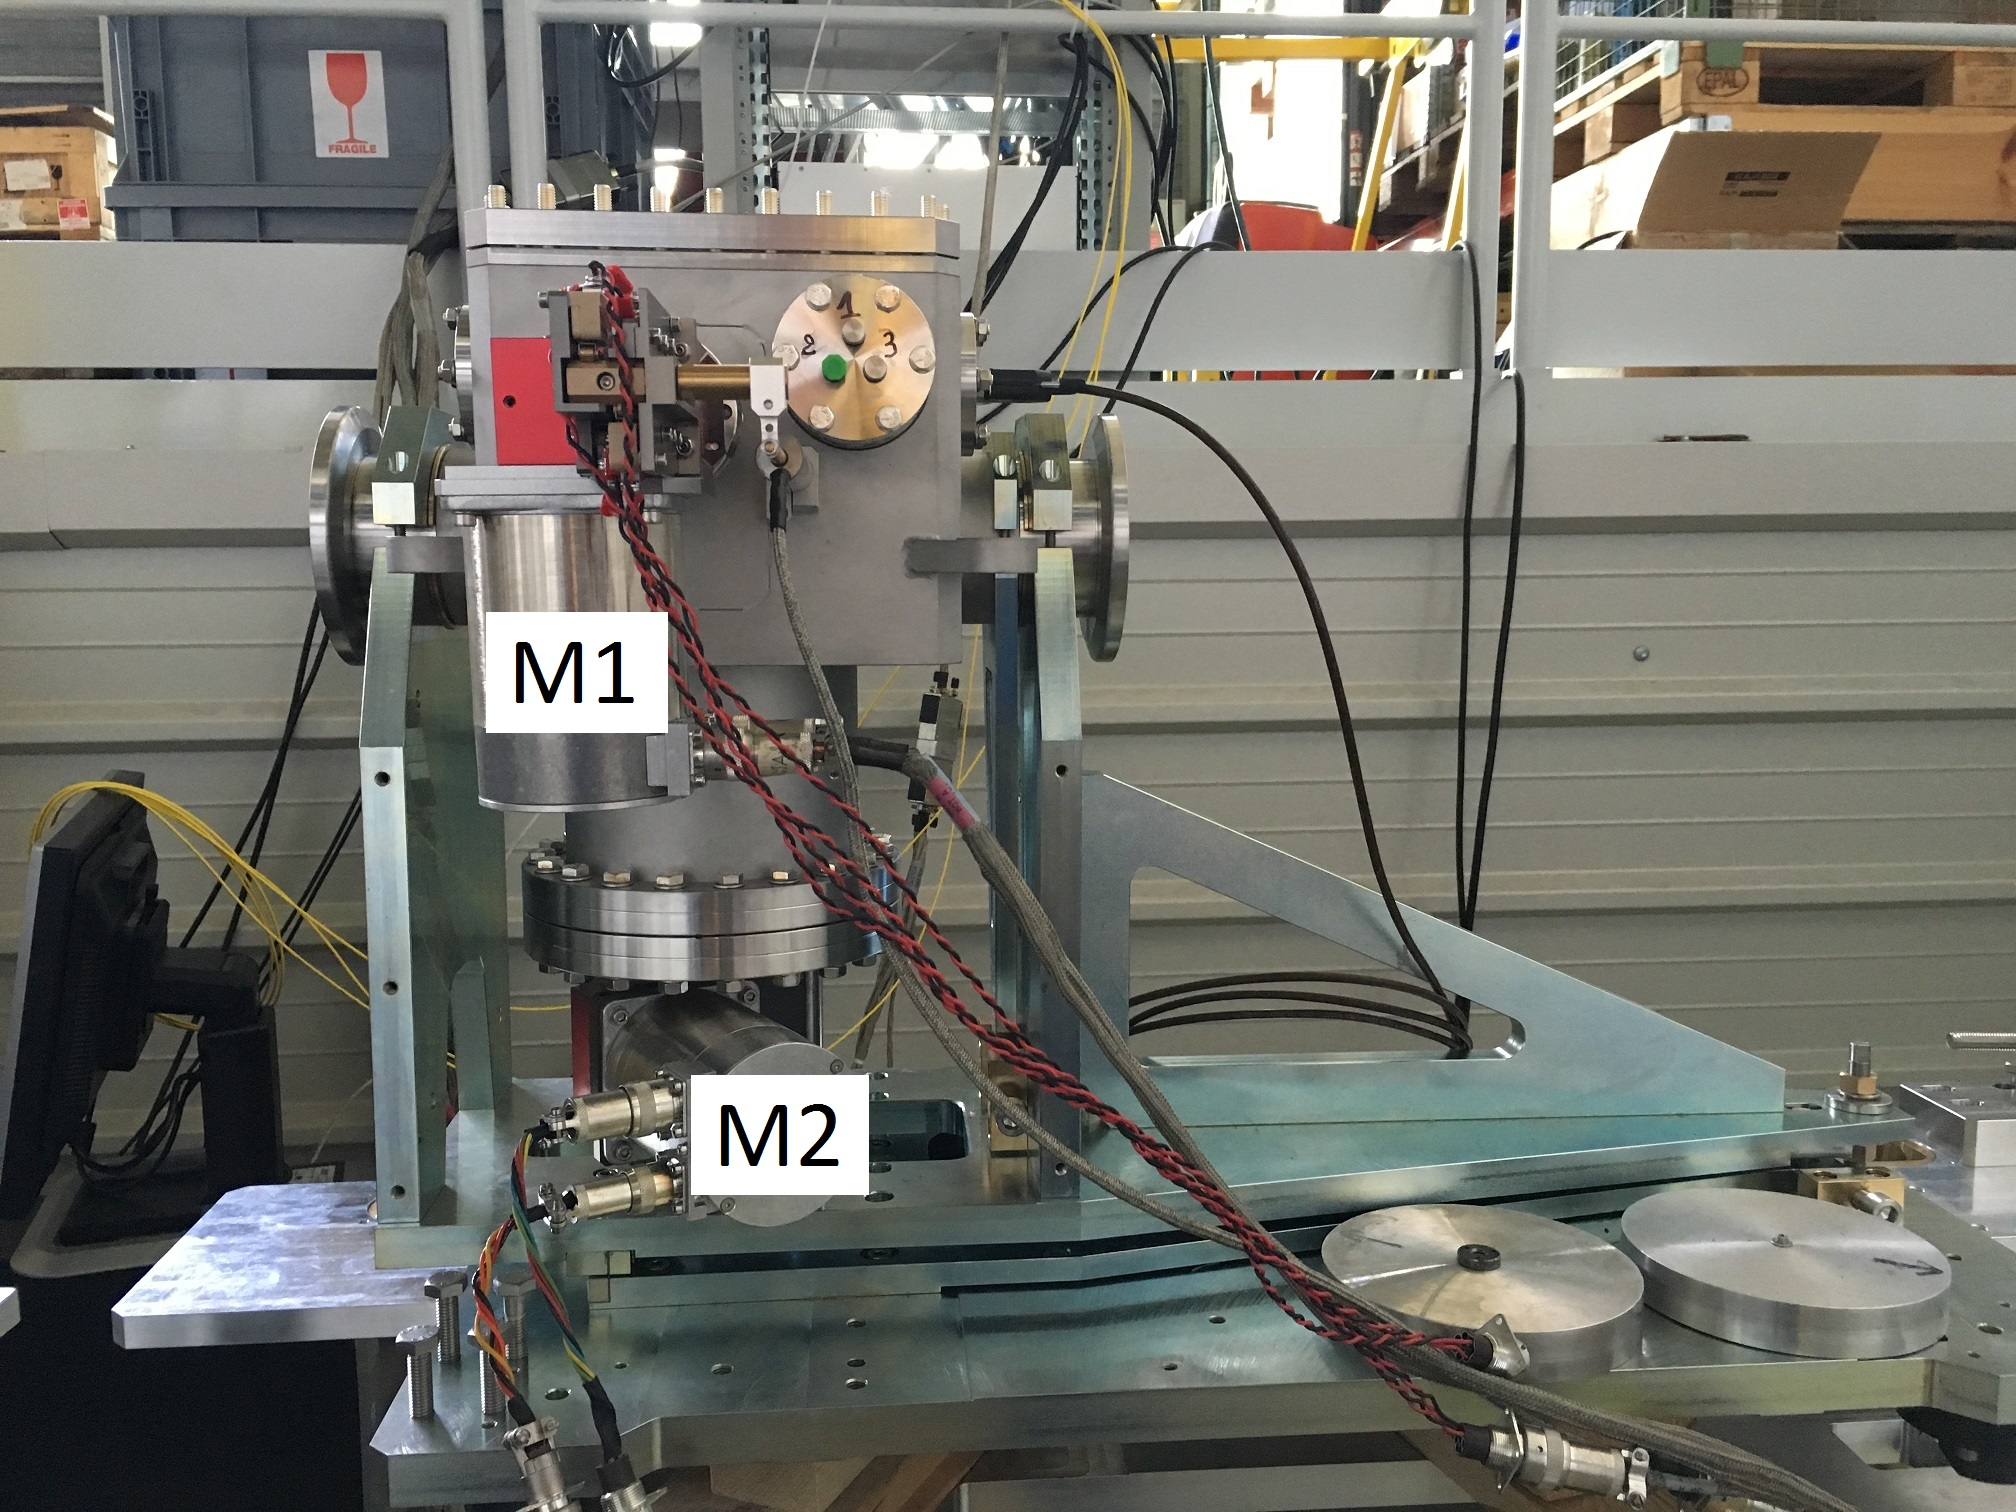
\includegraphics[width=0.5\textwidth, trim=10cm 12cm 50cm 7cm, clip=true]{fig/collimator-side}}
   \qquad
   \subfloat[][\label{fig:collimator-top}Collimator from top]{
   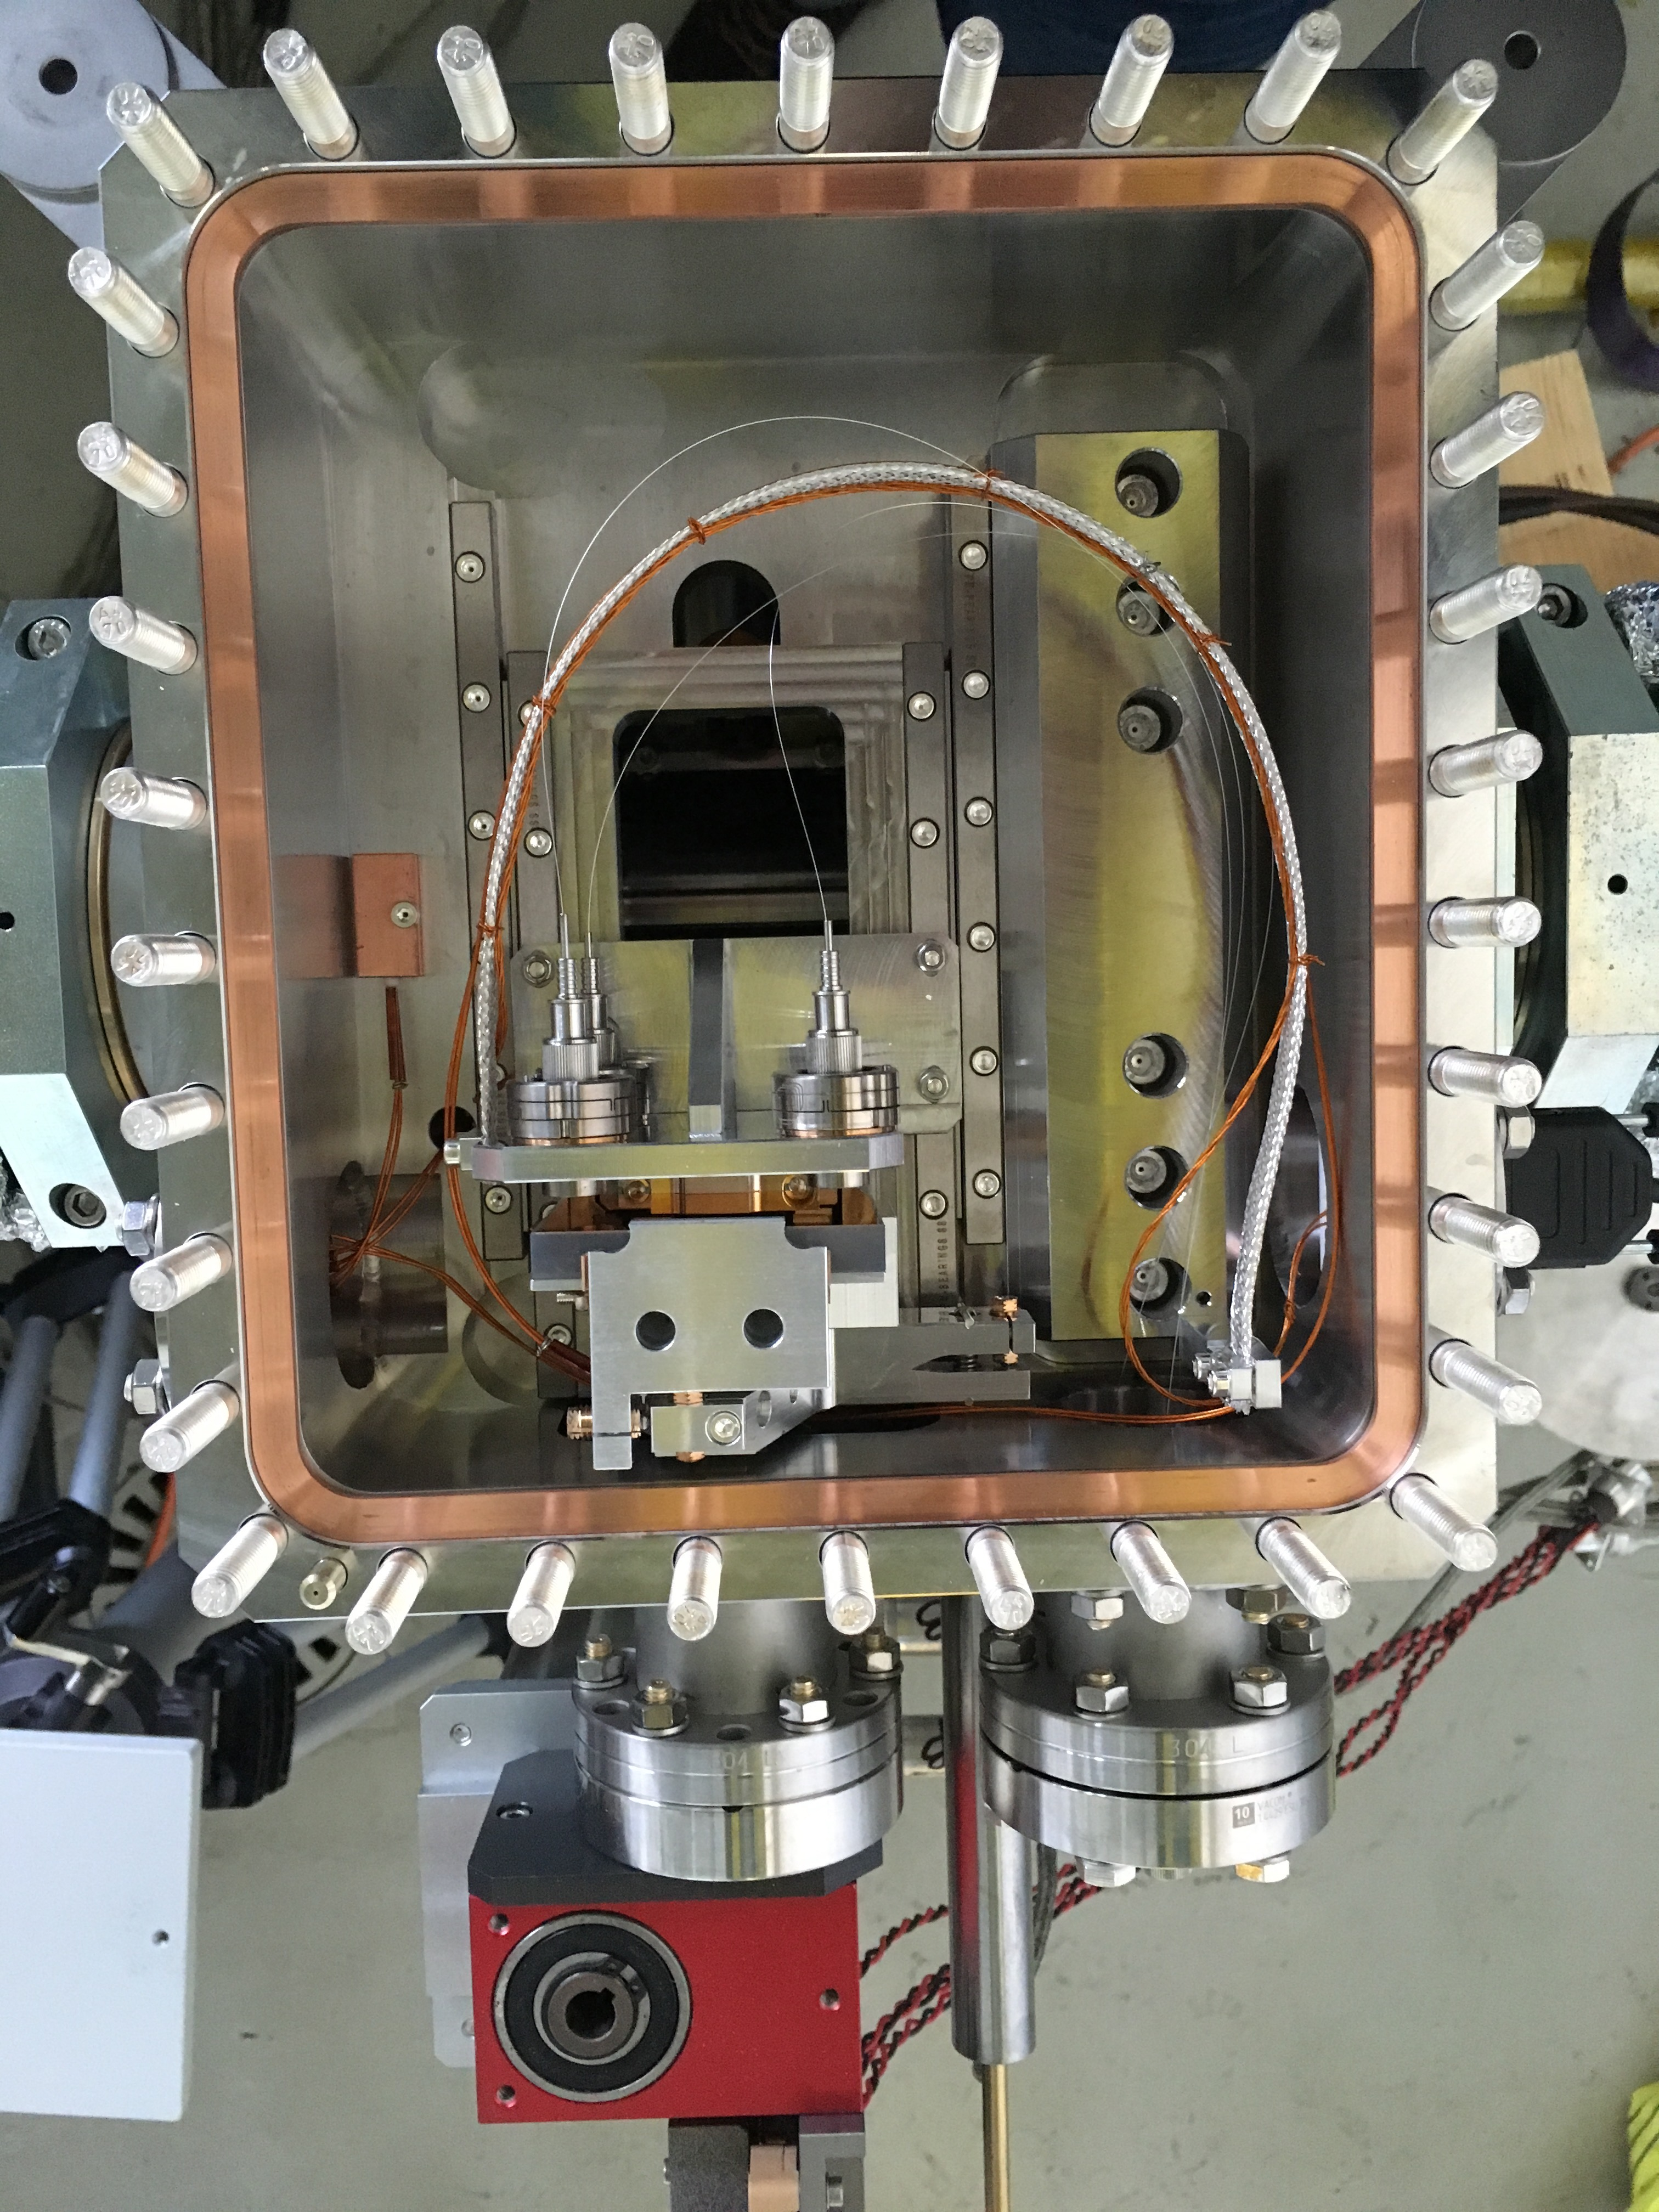
\includegraphics[width=0.4\textwidth, trim=0cm 0cm 0cm 0cm, clip=true]{fig/collimator-top}}
   \caption{\label{fig:collimator} Illustrates the collimator from the side (a) and the top (b).}
 \end{figure}



\section{Rotational stage}

\section{Piezoelectric stack actuator}

\section{System identification}
